Theatre is considered as lively art~\cite{wilson2009theatre}. Thanks its characteristics and constraints, it is an excellent framework to test sociability and expressiveness in robots; moreover, actor training systems (e.g.,~\cite{wilson2009theatre,cavanaugh2012acting,genevieve2009delsarte,Stanislavski1989} can inspire the development of expressive robots.
%%%%%%%%%%%%%%%%%%%%%%%%%%%%%%%%%
\subsection{Characteristics}
People are used to think at theatre as a repetitive show, and essential points that make theatre a lively art are often forgotten~\cite{wilson2009theatre}: 
\begin{itemize}
\item On the opposite of television or movies, during a theatre performance actors do not have a second chance to perform in front of the same audience. If an actor fails remembering a line, or he/she does not show a believable character, the audience are going to get a bad impression of the play.
\item Each performance is unique. No matter how much effort actors do to repeat each time the same performance, subtle changes could be seen: actors' and objects' stage position, actors' mood and, more importantly, audience's attitude. 
\item Audience's attitude affects actors. Actor could hear laughs, coughs, silence, and could even feel the tension in the audience. This could eager or discourage actors, affecting the whole performance. 
\item The performance outcome does not rely on one person. Good outcome comes from correct collaboration and coordination of playwriter, director, technical people and performers. In the specific performers case, they must work as a unity and show to the public a coherent story. 
\end{itemize}
Therefore, theatrical robot actors should have abilities similar to those of their human counterpart to be considered as actors and not as props. This makes necessary that robot actors be expressive, social, and with enough autonomy to be able to face anything may happen on stage.
%%%%%%%%%%%%%%%%%%%%%%%%%%%%%%%%%
\subsection{Constraints}
Theatre constraints makes it possible to focus research efforts on emotion expression and social behavior, considering that robots have already at least a general idea of what to do and how. These constraints are: 
\begin{itemize}
	\item The play script contains all the necessary information: actions, coordination cues, dialogues, and characters attitude. 
	\item Since the script is known before any representation, rehearsals can be done to get used with objects' and performers' positions.
	\item The stage space is discretized to facilitate directors to give instructions, and actors to remember their positions (Figure \ref{fig:StageDirections}).
\begin{figure}
	\centering
	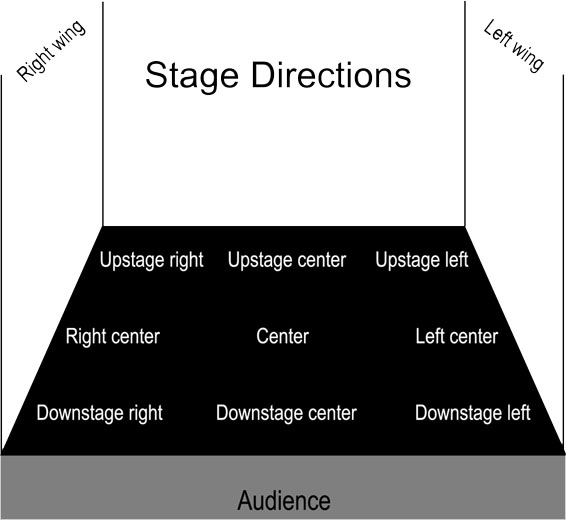
\includegraphics[width=0.4\textwidth]{Images/StageDirection.png} 
	\caption{Stage division used by directors to give instructions~\cite{Musical}.}
	\label{fig:StageDirections}
\end{figure}
	\item Actors should basically take one out of eight preset orientations during a performance (Figure~\ref{fig:BodyPosition}).   
	\begin{figure}
	\centering
	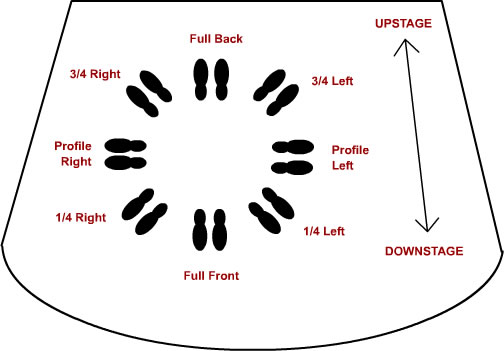
\includegraphics[width=0.4\textwidth]{Images/BodyPosition.png} 
	\caption{Eight possible actors' body position~\cite{Artopia}.}
	\label{fig:BodyPosition}
\end{figure}
\end{itemize}